\documentclass[10pt,a4paper]{amsart}
\usepackage[latin1]{inputenc}
\usepackage{mathtools} 
\usepackage{amssymb} 
\usepackage{mathrsfs} % gives mathscr font 
\usepackage{graphicx}
%\usepackage[headsep=0.15in, left=0.5in, right=0.5in, top=0.6in, bottom=0.5in]{geometry} 
%\usepackage[textlf,mathlf]{MinionPro} 
\usepackage{fancyhdr}
%\usepackage{xypic}
\usepackage{tikz-cd} 
\usepackage{todonotes}
\usepackage{verbatim}
\usepackage{filecontents}
\usepackage[colorlinks=true]{hyperref}
\usepackage{tabu}
\usepackage{multicol}
\usepackage{booktabs}
\usepackage{centernot}
\usepackage{bbm} % for blackboard bold 1 indicator functions
\usepackage{multirow}
\usepackage{enumerate}
\usepackage{stmaryrd} % for \mapsfrom
\usepackage{blkarray} % for labeled matrix

\definecolor{zaffre}{rgb}{0.0, 0.08, 0.66}
\hypersetup{colorlinks=true,allcolors=zaffre}

%Environments
\numberwithin{equation}{section} 
\numberwithin{figure}{section}
\numberwithin{table}{section}
\theoremstyle{definition} 
\theoremstyle{plain} 
\newtheorem{thm}{\protect\theoremname}[section]
\theoremstyle{definition}
\newtheorem*{alg}{Algorithm}
\newtheorem{subalg}{Subalgorithm}[section]
\newtheorem{example}[thm]{\protect\examplename}
\theoremstyle{remark} 
\newtheorem{rem}[thm]{\protect\remarkname}
\theoremstyle{plain}
\newtheorem{cor}[thm]{\protect\corollaryname}
\theoremstyle{definition} 
\newtheorem{defn}[thm]{\protect\definitionname}
\theoremstyle{plain} 
\newtheorem{prop}[thm]{\protect\propositionname}
\theoremstyle{plain} 
\newtheorem{lem}[thm]{\protect\lemmaname}
\newtheorem{conj}[thm]{Conjecture}
\theoremstyle{definition}
\newtheorem{notation}[thm]{Notation}

\providecommand{\definitionname}{Definition}
\providecommand{\examplename}{Example} 
\providecommand{\lemmaname}{Lemma}
\providecommand{\propositionname}{Proposition}
\providecommand{\remarkname}{Remark} 
\providecommand{\corollaryname}{Corollary}
\providecommand{\theoremname}{Theorem}

\setcounter{tocdepth}{1}

%macros, etc.
\newcommand{\legendre}[2]{\genfrac{(}{)}{}{}{#1}{#2}}
\renewcommand{\arraystretch}{1.2} 

\newcommand{\A}{\mathbb{A}}
\renewcommand{\P}{\mathbb{P}} 
\newcommand{\F}{\mathbb{F}}
\newcommand{\Z}{\mathbb{Z}}
\newcommand{\Q}{\mathbb{Q}}
\newcommand{\R}{\mathbb{R}}
\newcommand{\C}{\mathbb{C}}
\newcommand{\GL}{\operatorname{GL}}
\newcommand{\Span}{\operatorname{Span}}
\newcommand{\trsp}[1]{{{#1}^{\top}\!\!}}
\newcommand{\ndiv}{\centernot|}
\newcommand{\IND}{\mathbbm{1}}
\DeclareMathOperator{\img}{im}
\newcommand{\red}{\mathrm{red}}
\newcommand{\gr}{\operatorname{gr}}

\begin{document}
	%\section*{info}
\begin{itemize}
	\item[Xianglong] This section will serve as a place for us to write general comments. (Of course, it will be omitted from submissions.) Currently I am working on the section for part (1) of the problem. I think I will write the recursion stuff for computing the number of solutions as an appendix.
\end{itemize}

	\title{The $\F_p$ Fourier transform of indicator functions of conical subsets}
	\author{Xianglong Ni, Oron Propp, Miguel Young }
	
	\maketitle

	\begin{abstract}
	    We explore a generalization of the Fourier transform to complex
	    functions defined on $\F_p$-vector spaces. To this end, we compute the Fourier
	    transforms of indicator functions of conical subsets of these vector spaces in several specific cases.
	\end{abstract}
	
	\tableofcontents

    \section{Introduction}

The \emph{Fourier transform} takes a function $f:\R\to\C$ and produces another
function, $\Phi(f):\R\to\C$, via the following integral transform:
\[ \Phi(f)(\lambda) = \int_\R e^{-2\pi i x \lambda} f(x)\, dx. \]
Conceptually, this takes a \emph{frequency} $\lambda$, which determines the ``pure sinusoid''
$e^{-2\pi i x \lambda}$, and convolves it with $f$ to extract the \emph{amplitude} of $f$ 
at that frequency. This is especially clear when $f$ represents a wave, such as an alternating
current through time or a quantum mechanical wavefunction. 

The Fourier transform generalizes to higher dimensions, too. If we now have a function
$f:\R^n\to\C$, we can express the pure sinusoid associated to $\lambda\in\R^n$ by 
$e^{-2\pi i x\cdot\lambda}$ (note the dot product). For a general real vector space $V$, where
we still have a notion of integration, it might be more natural to define the 
Fourier transform as a function from the dual, $V^* \to \C$, given by
\[ \Phi(f)(\lambda) = \int_\R e^{-2\pi i \lambda(x)} f(x)\, dx. \]
This is the same transform described for $\R^n$; every linear functional from $\R^n$ is
just given by a dot product. In all of the cases outlined above, a pure sinusoid, or
\emph{character}, sends addition to multiplication. In fact, it's a group homomorphism 
$\lambda:V \to \C^\times$, where we require that $|\lambda(x)| = 1$ for all $x\in V$.

In fact, we don't need to stick to real analysis to preform Fourier transforms; they're
valid wherever we have a notion of \emph{characters}
and \emph{integration}. A familiar object with both of these properties is the finite field
$\F_p$, as we will show. Our choice of integration is easy: given any $f:\F_p\to\C$, we define
\[ \int_{\F_p} f(x)\, dx = \sum_{x\in\F_p} f(x). \]
It's a linear map, and respects translation: $f(x + n)$, $n$ fixed, integrates to the 
same value as $f(x)$. Characters require just a bit more thinking: to give a character 
$\lambda$, we need to give a complex number whose $p$th power is $1$, that is, we need
to chose a root of unity. So we have a formula for the set of characters:
\[ \lambda(x) = \exp {\frac{2\pi i}{p} x \lambda}, \]
where we've identified the character $\lambda$ with the element $\lambda\in\F_p$, by
abuse of notation. Applying a generalization like for $\R^n$, we can define a general
finite Fourier transform.
\begin{defn}
    Let $V$ be any $\F_p$-vector space, and $f:V\to \C$ be any function. The Fourier
    transform is a function $\Phi(f):V^*\to\C$, defined on the dual space, given by
    \[ \Phi(f)(\lambda) = 
        \sum_{x\in\F_p} \exp \left(\frac{2\pi i}{p} \lambda(x)\right) f(x). \]
\end{defn}

Our goal is to explore the effect of this transform on \emph{indicator functions}; for
some fixed $\F_p$-vector space $V$, and a subset $S\subset V$, define
\[ \IND_S(x) = \begin{cases}
    1 & x \in V \\
    0 & \text{otherwise}     
\end{cases} \]
In this situation, the Fourier transform is somewhat simpler, and is entirely
determined by what a functional $\lambda$ does on the subset $S$.
\[ \Phi(\IND_S)(\lambda) = \sum_{x\in S} \exp \left(\frac{2\pi i}{p} \lambda(x)\right). \]
Noting that $\IND_S = 1 - \IND_{V\setminus S}$, we can write the Fourier transform as
\[ \Phi(\IND_S)(\lambda) = 1 - \sum_{x\not\in S} \exp \left(\frac{2\pi i}{p} \lambda(x)\right), \]
which will be occasionally convenient. 

\begin{rem}
    Throughout, for each vector space $V$, we implicitly pick an isomorphism 
    $V\cong\F_p^n$, i.e., an explicit basis. This
    entitles us to an inner product on $V$, as well as an isomorphism between $V$ and
    $V^*$, where all functionals are of the form $x \mapsto \langle \lambda, x \rangle$
    for some $\lambda\in V$. By abuse of notation, $\lambda$ also denotes the functional.
\end{rem}

TODO: summary of results.
    \section{$S$ is a linear subspace of $V$}\label{sec:part0}
\textcolor{red}{moved some stuff here from first section, will edit some later---need to put lemma in here somewhere}

In this situation, the Fourier transform is somewhat simpler, and is entirely
determined by what a functional $\lambda$ does on the subset $S$.
\[ \Phi(\IND_S)(\lambda) = \sum_{x\in S} \exp \left(\frac{2\pi i}{p} \lambda(x)\right). \]
Noting that $\IND_S = 1 - \IND_{V\setminus S}$, we can write the Fourier transform as
\[ \Phi(\IND_S)(\lambda) = 1 - \sum_{x\not\in S} \exp \left(\frac{2\pi i}{p} \lambda(x)\right), \]
which will be occasionally convenient. 

\begin{rem}
	Throughout, for each vector space $V$, we implicitly pick an isomorphism 
	$V\cong\F_p^n$, i.e., an explicit basis. This
	entitles us to an inner product on $V$, as well as an isomorphism between $V$ and
	$V^*$, where all functionals are of the form $x \mapsto \langle \lambda, x \rangle$
	for some $\lambda\in V$. By abuse of notation, $\lambda$ also denotes the functional.
\end{rem}

Let us being with a warmup. Consider the case of a subspace $W$ of our vector space $V$.
A classical theorem of linear algebra allows us to decompose $V$:
\begin{prop}
    The \emph{orthogonal complement} of $W$ is the subspace    
    \[ W^\perp = \{ v \in V \,|\, \langle v, w \rangle = 0 \text{ for all } w \in W \}. \]
    Any element $x\in V$ may be uniquely written as a sum $x = w + w'$, where $w\in W$
    and $w'\in W^\perp$.
\end{prop}

Before we consider the Fourier transform over the whole space $V$, consider what
it does to elements of $W$:
\begin{lem}
    \label{lem:subspace-transform-on-subspace}
    Suppose $\lambda\in W$ is nonzero. Then, $\Phi(\IND_W)(\lambda) = 0$.
    \begin{proof}
        We prove this by induction on the dimension of $W$. Fix any element $w\in W$,
        and let $U\subset W$ be the line spanned by it. Then,   
        \[ \Phi(\IND_W)(\lambda) = 
            \sum_{x\in W/U} 
                \exp \left(\frac{2\pi i}{p} \langle \lambda, x \rangle\right) +
            \sum_{x\in U} 
                \exp \left(\frac{2\pi i}{p} \langle \lambda, x \rangle\right). \]
        It is easy to see that the rightmost term is zero:
        \[ \sum_{x\in U} 
                \exp \left(\frac{2\pi i}{p} \langle \lambda, x \rangle\right) =
            \sum_{x\in \F_p} 
                \exp \left(\frac{2\pi i}{p} x \langle \lambda, w \rangle\right) = 0,
                \]
        since $\langle \lambda, w \rangle \neq 0$. Since the dimension of $W/U$ is less
        than that of $W$, we can continue repeating this process until there's nothing left.
    \end{proof}
\end{lem}
We can now put these facts together to prove our result:
\begin{thm}
    $\Phi(\IND_W) = |W| \IND_{W^\perp}$.
    \begin{proof}
        Given $\lambda\in V$, split it into orthogonal parts as $\lambda = w + w'$. Then,
        \[ \Phi(\IND_W)(w + w') = 
            \sum_{x\in W} 
                \exp \left(\frac{2\pi i}{p} \langle w + w', x \rangle\right) = 
            \sum_{x\in W} 
                \exp \left(\frac{2\pi i}{p} \langle w, x \rangle\right). \]
        If $w\neq 0$, by Lemma \ref{lem:subspace-transform-on-subspace}, the whole
        sum will vanish; otherwise, the exponent will be constantly $1$, and add up to
        $|W|$. In the case that $w = 0$, $\lambda\in W^\perp$, as desired.
    \end{proof}
\end{thm}
TODO: geometric intution?

	\section{Homogeneous quadratics in $n$ variables}\label{sec:part1}
Having established the needed groundwork in the preceding section, we move on to computing examples of the Fourier transform $\Phi(\IND_S)$. In this section we consider the case when $V = \F_p^n$ and
\[
	S = \{(x_1,\ldots,x_n) \mid Q(x_1,\ldots,x_n) = 0\}
\]
where $Q$ is a homogeneous quadratic. In order to compute $\Phi(\IND_S)$ using Lemma \ref{lem:FT-conical-subset}, we must determine $|\ker \lambda \cap S|$ given a $\lambda \in V^*$. If we think of elements of $V$ as column vectors, then elements $\lambda \in V^*$ can be thought of as row vectors, with
\[
	\ker \lambda = \langle \lambda \rangle^\bot = \{x \in V \mid \lambda x =0\}.
\]

We begin with an illustrative example over the reals before considering the situation over $\F_p$. Let $Q = 3x_1^2 + 3x_2^2 - 2x_3^2$. The quadric $S = \{Q = 0\}$ is depicted in Figure~\ref{fig:conic-with-plane}.
\begin{figure}[h]
	\centering
	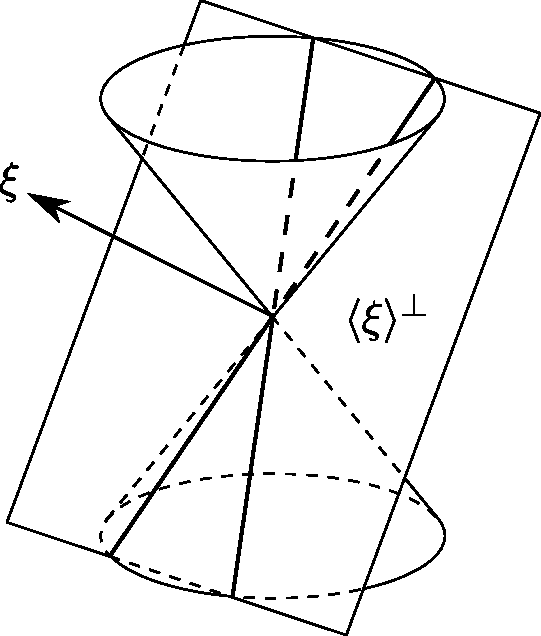
\includegraphics[width=0.6\linewidth]{conic-with-plane}
	\caption{}
	\label{fig:conic-with-plane}
\end{figure}
The intersection $\langle \lambda \rangle^\bot \cap S$ has three possible shapes:
\begin{itemize}
	\item a pair of lines intersecting at the origin (which is the case depicted with $\lambda = (0,-2,1)$),
	\item the origin alone (e.g. $\lambda = (0,0,1)$), and
	\item a single line, which happens when $\langle \lambda \rangle^\bot$ is tangent to the quadric (e.g. $\lambda = (0,-\sqrt{3},\sqrt{2})$).
\end{itemize}
In fact, the set of $\lambda$ such that $\langle \lambda \rangle^\bot$ is tangent to the quadric is given by
\[
	\left\{ \lambda = (\lambda_1,\lambda_2,\lambda_3) \mid \frac{1}{3} \lambda_1^2 + \frac{1}{3} \lambda_2^2 - \frac{1}{2} \lambda_3^2 = 0 \right\} \subset V^*.
\]
This is a quadric in $V^*$, and it is dual to our original quadric in a sense that we will soon explain. Let us we write $Q^*$ for the equation of this dual quadric. Observe that $Q^*(0,-2,1) > 0$ while $Q^*(0,0,1) < 0$. It turns out that the sign of $Q^*(\lambda)$ is all one needs to classify the intersection $\langle \lambda \rangle^\bot \cap S$. Equivalently, one needs only consider the existence of square-roots of $Q^*(\lambda)$---a notion which, unlike ``sign,'' still makes sense over $\F_p$.

Now we consider the general situation in $n$ variables over a field $k$. We will require that $\operatorname{char} k \neq 2$, and that the product of two non-squares in $k$ is a square. The fields $\Q$, $\R$, and $\F_p$ for $p>2$ are examples. To a homogeneous quadratic
\[
	Q = \sum_{1 \leq i \leq j \leq n} c_{i,j} x_i x_j 
\]
we associate the $n\times n$ matrix $A$ whose entries are given by
\[
	a_{i,j} = \begin{cases}
		{c_{i,j}}/{2} & \text{if } i < j,\\
		c_{i,j} & \text{if } i = j, \text{ and}\\
		{c_{j,i}}/{2} & \text{if } i > j.
	\end{cases}
\]
Then, if $x = (x_1,\ldots,x_n)^\top$, we have
\[
	Q(x) = x^\top A x.
\]
The quadric $S = \{Q = 0\}$ is \emph{non-degenerate} if the matrix $A$ is invertible. We will assume that this is the case.

\begin{defn}
	The \emph{orthogonal group of $A$}, denoted $O(A)$, is defined to be
	\[
		O(A) \coloneqq \{ g \in GL(V) \mid g^\top A g = A\}.
	\]
	Also define
	\[
		kO(A) \coloneqq \{ cg \mid c\in k, g\in O(A)\}.
	\]
\end{defn}

We are interested in this group because elements of $kO(A)$ map $S$ to itself.
\begin{defn}
	A group $G$ acts \emph{transitively} on a set $X$ if for all $a,b\in X$, there exists $g\in G$ such that $g\cdot a = b$. Equivalently, the only orbit of the action is the entirety of $X$.
\end{defn}

\begin{prop}\label{prop:OA-transitive-action}
	The group $kO(A)$ acts transitively on each of the following sets:
	\begin{enumerate}
		\item $S_0(A) \coloneqq \{x \in V \mid x\neq 0, x^\top A x = 0\}$,
		\item $S_+(A) \coloneqq \{ x\in V \mid x^\top A x \text{ is a nonzero square in } k\}$, and
		\item $S_-(A) \coloneqq \{ x\in V \mid x^\top A x \text{ is not a square in } k\}$.
	\end{enumerate}
\end{prop}
\begin{proof}
	If $u,v\in V$ belong to the same set above, we can assume $u^\top A u = v^\top A v$ (as it can be achieved by scaling). This relies on our assumption that the quotient of two non-squares is a square in $k$.
	
	If $u$ and $v$ are linearly dependent then the result is immediate, so suppose otherwise. Take a basis $\{u,v,e_3,\ldots,e_n\}$ and apply Gram-Schmidt to it, obtaining an orthogonal basis $\{u, w_2, w_3, \ldots,w_n\}$. Now consider the basis
	\[
		\{u,v,w_3,\ldots,w_n\}
	\]
	which has the property that
	\[
		w_i^\top A u = w_i^\top A v = w_i^\top A w_j = 0 \text{ for all } i \neq j, \text{ and }\\
		u^\top A u = v^\top A v.
	\]
	It is straightforward to verify that the linear transformation which interchanges $u$ and $v$ while fixing $w_3,\ldots,w_n$ is an element of $O(A)$.
\end{proof}

Note that left-multiplication by an element $g \in O(A)$ on $V$ induces right-multiplication by $g^{-1}$ on $V^*$.

Now suppose that $\lambda^\top,\lambda'^\top$ both belong to $S_0(A^{-1})$ (the following argument applies for the other two sets in Proposition \ref{prop:OA-transitive-action} as well). Then there exists $g \in O(A^{-1})$ such that $g \lambda^\top = \lambda'^\top$. If $\lambda x = 0$, then
\[
	\lambda' (g^\top)^{-1} x = \lambda x = 0
\]
and thus $(g^\top)^{-1}$ maps $\langle \lambda \rangle^\bot$ to $\langle \lambda' \rangle^\bot$. Moreover, since $g \in O(A^{-1})$, inverting the identity $g^\top A^{-1} g = A^{-1}$ shows that $(g^\top)^{-1} \in O(A)$.

Thus we get a map
\[
	(g^\top)^{-1} \colon S \cap \langle \lambda \rangle^\bot \to S \cap \langle \lambda' \rangle^\bot
\]
which is a bijection.

Specializing back to $k=\F_p$ for $p>2$ a prime, we conclude that $\Phi(\IND_S)$ assumes only a few values.

\begin{thm}\label{thm:FT-quadratic-constants-TBD}
	Let $p > 2$ be a prime and let $Q(x_1,\ldots,x_n)$ be a homogeneous non-degenerate quadratic. Write $S$ for the quadric $\{Q = 0\}$ in $V=\F_p^n$. Then,
	\begin{equation}
	\Phi(\IND_S)(\lambda) = \begin{cases}
	\Phi(\IND_S)(0) & \text{if } \lambda = 0,\\
	N_0 & \text{if } \lambda \in S_0(A^{-1}),\\
	N_+ & \text{if } \lambda \in S_+(A^{-1}), \text{ and}\\
	N_- & \text{if } \lambda \in S_-(A^{-1}),
	\end{cases}
	\end{equation}
	for some constants $N_0$, $N_+$, and $N_-$.
\end{thm}
Let $Q^*$ be the quadratic given by
\[
	Q^*(\lambda) = \lambda A^{-1} \lambda^\top.
\]
Then the above equivalently states that for nonzero $\lambda$, the value of $\Phi(\IND_S)(\lambda)$ depends only on the number of square roots of $Q^*(\lambda)$.

Now we compute the constants in Theorem \ref{thm:FT-quadratic-constants-TBD}. It is a well-known fact (see for example \cite[Prop.~42:1]{omeara}) that there exists an invertible $n\times n$ matrix $P$ such that $P^\top A P$ is diagonal. The matrix $P$ defines a change of coordinates, where in the new coordinates the equation of the quadric is
\[
x^\top P^\top A P x = 0.
\]
Since $P^\top A P$ is diagonal, this equation takes the form
\[
c_1 x_1^2 + c_2 x_2^2 + \cdots + c_n x_n^2 = 0
\]
where all the $c_i$ are nonzero because we assumed $A$ to be invertible.

Fix a non-square $r\in \F_p$. For each $c_i$, either $c_i$ is a square or $c_i / r$ is a square. By scaling the coordinates as needed, we can assume that each $c_i$ is either $1$ or $r$.

There exists an $a\in\F_p$ such that $a^2 + 1$ is a non-square. Suppose that for distinct $i,j\in\{1,\ldots,n\}$ the coefficients of $x_i$ and $x_j$ are both $r$. We can apply the invertible transformation which replaces $x_i$ by $ax_i + x_j$ and $x_j$ by $x_i - ax_j$ in the equation for the quadric, and this turns the expression $rx_i^2 + rx_j^2$ into $r(a^2 + 1)x_i^2 + r(a^2+1)x_j^2$. As the product of two non-squares, these new coefficients are squares. Hence we may assume that they are equal to $1$.

This shows that we can reduce to the two following forms:
\begin{align}
x_1^2 + x_2^2 + \cdots + x_n^2 &= 0\text{ or} \tag{Q1}\label{eq:Q1}\\ 
rx_1^2 + x_2^2 + \cdots + x_n^2 &= 0. \tag{Q2}\label{eq:Q2}
\end{align}
In Appendix \ref{sec:recursion-for-quadratic-solns} we give recursions $f_n, g_n$ for computing the number of solutions to such equations. We conclude this section by giving an example of how to compute the constants in Theorem \ref{thm:FT-quadratic-constants-TBD} from $f_n$ and $g_n$.

\begin{example}
	Suppose our equation is to the form \eqref{eq:Q1} and $-1$ is a square mod $p$. Then $\Phi(\IND_S)(0)$ is the total number of points on the quadric, which in this case is $f_n (0)$:
	\[
		\Phi(\IND_S)(0) = f_n(0).
	\]
	To compute $N_0$, observe that \eqref{eq:Q1} is equivalent to
	\[
		-x_1^2 + x_2^2 + \cdots + x_n^2 = 0
	\]
	because $-1$ is a square. Consider $\lambda = (1,1,0,0,\ldots,0)$. Its kernel is the hyperplane $\{x_1 + x_2 = 0\}$. Substituting $x_1 = -x_2$ into the above gives
	\[
	x_3^2 + \cdots + x_n^2 = 0.
	\]
	This has $p f_{n-2}(0)$ solutions in the variables $x_2,\ldots,x_n$. Thus
	\[
	N_0 = \frac{p^2 f_{n-2}(0) - f_n(0)}{p-1}.
	\]
	To compute $N_+$, consider $\lambda = (1,0,0,\ldots,0)$ whose kernel is the hyperplane $\{x_1 = 0\}$. Substituting this into \eqref{eq:Q1} gives
	\[
	x_2^2 + x_3^2 \cdots + x_n^2 = 0
	\]
	which has $f_{n-1}(0)$ solutions in the variables $x_2,x_3,\ldots,x_n$, and thus
	\[
	N_+ = \frac{p f_{n-1}(0) - f_n(0)}{p-1}.
	\]
	Finally, to compute $N_-$, we note that \eqref{eq:Q1} is also equivalent to the quadric
	\[
		rx_1^2 + rx_2^2 + x_3^2 + \cdots + x_n^2 = 0
	\]
	and we can take $\lambda = (1,0,0,\ldots,0)$ and consider the intersection of its kernel with this quadric. Setting $\{x_1 = 0\}$ gives the equation
	\[
		rx_2^2 + x_3^2 + \cdots + x_n^2 = 0
	\]
	which has $g_{n-1}(0)$ solutions, and hence
	\[
		N_- = \frac{pg_{n-1}(0) - f_n(0)}{p-1}.
	\]
	If $n$ is even, then $f_{n-1}(0) = g_{n-1}(0)$ (c.f. Appendix \ref{sec:recursion-for-quadratic-solns}) and thus $N_+ = N_-$.
\end{example}
	\section{Homogeneous polynomials in 2 variables}\label{sec:part2}
In the preceding section, we considered degree $2$ homogeneous polynomials in $n$ variables. Now we will instead consider degree $n$ homogeneous polynomials in $2$ variables. However, we will set things up quite differently.

Let $\F_p[x,y]_n$ denote the space of homogeneous polynomials of degree $n$ over $\F_p$. It is an $(n+1)$-dimensional vector space, spanned by the basis elements
\[
	\{x^n, x^{n-1}y, \ldots, xy^{n-1}, y^n\}.
\]
Now define $V$ to be the dual space of this vector space:
\[
	V \coloneqq \left(\F_p[x,y]_n\right)^*.
\]
Of particular algebraic interest are the elements of $V$ which are given by \emph{evaluation} at a point---these are the functionals $ev_{a,b}\colon \F_p[x,y]_n \to \F_p$ of the form
\[
	ev_{a,b}(P) = P(a,b) 
\]
for some $a,b\in \F_p$.

However, the set of all $ev_{a,b}$ need not be conical: consider
\[
	2ev_{1,0} \in \F_3[x,y]_2.
\]
This functional at $P(x,y) = x^2$ takes the value $2$, but $2\in \F_3$ is not a square and thus $2ev_{1,0}$ cannot be equal to $ev_{a,b}$ for any $a,b\in \F_3$. To get around this, we will instead let $S$ be the set
\[
	S=\{\xi_{a,b,c} \in V \mid \xi_{a,b,c}(P) = cP(a,b)\}.
\]
The Fourier transform of $\IND_S$ will be a $\C$-valued function on $V^*$, where $V^*$ is the double dual of $\F_p[x,y]_n$. Since $\F_p[x,y]_n$ is finite-dimensional, it is canonically isomorphic to its double dual, so we will identify $V^* = \F_p[x,y]_n$.

Define $\P^1$ to be the set of lines through the origin in $\F_p^2$. For each line $\ell \in \P^1$, pick a nonzero point $(a_\ell,b_\ell)$ on $\ell$. Then we have
\begin{equation}\label{eq:part2S}
	S = \{0\} \cup \{\xi_{a_\ell,b_\ell,c} \mid c\in \F_p \text{ nonzero}, \ell \in \P^1 \}
\end{equation}
and hence
\[
	|S| = 1 + (p+1)(p-1) = p^2.
\]
We will now give a very simple description of $\widehat{\IND_S}$.
\begin{thm}\label{thm:part2thm}
	Let $\F_p[x,y]_n$ be the space of homogeneous polynomials of degree $n$ over $\F_p$, $V$ its dual space, and $S\subset V$ the set $\{\xi_{a,b,c} \in V \mid \xi_{a,b,c}(P) = cP(a,b)\}$.
	
	An element $\xi \in V^*$ is a polynomial $P(x,y)$. Let $N_\xi$ be the number of solutions to $P(x,y)=0$ in $\F_p^2$. Then
	\begin{equation}
		\widehat{\IND_S}(\xi) = \frac{pN_\xi - p^2}{p-1}.\label{eq:FTpart2}
	\end{equation}
\end{thm}
\begin{proof}
	An element $\xi_{a,b,c}\in S$ is in $\ker \xi$ when $P(a,b) = 0$. From \eqref{eq:part2S}, we have
	\[
		|S \cap \ker \xi| = N_\xi
	\]
	and thus, by Lemma \ref{lem:FT-conical-subset},
	\begin{align*}
		\widehat{\IND_S}(\xi) &= \frac{p|S\cap \ker \xi| - |S|}{p-1}\\
		&= \frac{pN_\xi - p^2}{p-1}.\qedhere
	\end{align*}
\end{proof}
There is unfortunately no explicit formula for the number $N_\xi$ of solutions to $P(x,y) = 0$ in terms of the coefficients of $P$, so we will not attempt to expand further on \eqref{eq:FTpart2}. Instead, we offer an alternative geometric perspective which also leads to a proof of Theorem \ref{thm:part2thm}. Each polynomial in $V^* = \F_p[x,y]_n$ can be thought of a row vector $(a_0,\ldots,a_n)$ where $a_i$ is the coefficient of $x^{n-i}y^i$ in the polynomial. Then ``evaluation at $(a,b)$'' is given by pairing with the column vector
\[
	(a^n,a^{n-1}b,\ldots,ab^{n-1},b^n)^\top.
\]
With this identification, $S = \{\xi_{a,b,c}\}$ is the union of the following lines:
\begin{align*}
	\ell_\infty &= \langle (0,0,\ldots,0,1)^\top \rangle,\\
	\ell_0 &= \langle (1,0,\ldots,0,0)^\top \rangle,\\
	\ell_1 &= \langle (1,1,\ldots,1,1)^\top \rangle,\\
	\ell_2 &= \langle (1,2,\ldots,2^{n-1},2^n)^\top \rangle,\\
	\vdots &= \vdots\\
	\ell_{p-1} &= \langle (1,p-1,\ldots,(p-1)^{n-1},(p-1)^n)^\top \rangle
\end{align*}
As an aside for the reader familiar with algebraic geometry, if we think of $S$ as living inside projective space $\P^{n}$, it is the \emph{rational normal curve} of degree $n$ over $\F_p$.

Using the fact that $S$ is the union of the above lines, we can write
\begin{align*}
	\widehat{\IND_S} &= \sum \widehat{\IND_{\ell_i}} - p\widehat{\IND_{\{0\}}} \\
	&= p\left(\sum \IND_{\ell_i^\bot} - \IND_{V^*}\right).
\end{align*}
where we have used the linearity of the Fourier transform together with Theorem \ref{thm:FT-subspace}. A polynomial $P$ is in $\ell_i^\bot$ when it vanishes on $\ell_i$. If $P$ vanishes at $N$ points in total, then it vanishes on $(N - 1)/(p-1)$ of the lines $\ell_i$. This gives another proof of Theorem \ref{thm:part2thm}.

What is the ``geometry'' of these hyperplanes $\ell_i^\bot$? If $n < p$ then clearly not all $p+1$ of the lines $\ell_i$ can be linearly independent. We claim, however, that every subset of size at most $n+1$ is indeed linearly independent. A way of seeing this is by noting that the Vandermonde determinant is nonzero. Alternatively, one can explicitly produce a polynomial $P \in \F_p[x,y]_n$ which vanishes on $n$ given lines but not on the others. On the other hand, if an element of $\F_p[x,y]_n$ vanishes on $n+1$ of the lines, then in fact it vanishes on all of the lines. This is entirely what we expect: dividing the polynomial by $y^n$ gives a univariate polynomial in $(x/y)$ of degree at most $n$. If such a polynomial has $n+1$ roots, then it is identically zero.

\textcolor{red}{need to add summary}
    \newcommand{\Mat}{\operatorname{Mat}}
\newcommand{\tr}{\operatorname{tr}}
\newcommand{\fact}{\operatorname{fact}}

\section{Nilpotent $n\times n$ matrices}\label{sec:part3}

Now we turn our attention to an example of a much different flavor: in this section, we consider the case where $V$ is the space of $n\times n$ matrices with entries in $\F_p$, and $S$ is the subset of all nilpotent matrices. We assume $n\ge 2$, as when $n=1$ the problem is trivial. As before, to compute $\Phi(\IND_S)$, we must determine $|\ker\lambda\cap S|$ for a given $\lambda\in V^*$. We begin by identifying $V^*$ with $V$ via the nondegenerate symmetric bilinear form
\begin{align*}
V\times V&\to\F_p,\\
(A,B)&\mapsto\tr(AB).
\end{align*}
Under this identification, $\lambda$ corresponds to a matrix $M_\lambda\in V$, and we have
\begin{equation}
\label{eqn:kerlambda}
\ker\lambda\cap S=\{A\in S:\tr(AM_\lambda)=0\}.
\end{equation}
Our goal is to describe the cardinality of this set in terms of the matrix $M_\lambda$.
\begin{lem}
\label{lem:sim}
The value $|\ker\lambda\cap S|$ depends only on $M_\lambda$ up to similarity.
\end{lem}
\begin{proof}
Let $P\in V$ be invertible. Then for any $A\in S$, we have
\begin{equation*}
\tr(AP^{-1}M_\lambda P)=\tr(PAP^{-1}M_\lambda),
\end{equation*}
so it suffices to show that the invertible elements of $V$ act on $S$ by conjugation. Indeed, since $A$ is nilpotent, there exists some $k>0$ such that $A^k=0$, whence
\begin{equation*}
(PAP^{-1})^k=PA^kP^{-1}=0
\end{equation*}
as well.
\end{proof}
This lemma allows us to replace $M_\lambda$ by any matrix similar to it, thus simplifying the set of matrices we must consider. Our next step is to obtain convenient representatives for the similarity classes in $V$.
\begin{notation}
Given a monic polynomial
\begin{equation*}
f(x)=a_0+a_1x+\cdots+a_{d-1}x^{d-1}+x^d,
\end{equation*}
its \emph{companion matrix} is the $d\times d$ matrix
\begin{equation*}
C(f)=\begin{bmatrix}
0&0&\cdots&0&-a_0\\
1&0&\cdots&0&-a_1\\
0&1&\cdots&0&-a_2\\
\vdots&\vdots&\ddots&\vdots&\vdots\\
0&0&\cdots&1&-a_{d-1}
\end{bmatrix}.
\end{equation*}
\end{notation}
\begin{thm}
\label{thm:rcf}
Let $M\in V$. There exists a unique invertible $P\in V$ such that $P^{-1}MP$ is of the block form
\begin{equation}
\label{eqn:rcf}
\begin{bmatrix}
C(f_1)&0&\cdots&0\\
0&C(f_2)&\cdots&0\\
\vdots&\vdots&\ddots&\vdots\\
0&0&\cdots&C(f_m)
\end{bmatrix}
\end{equation}
for monic polynomials $f_1,\ldots,f_m\in\F_p[x]$. We say that such a matrix is in \emph{rational canonical form}. Moreover, the polynomials $f_1,\ldots,f_m$, called the \emph{invariant factors} of $M$, satisfy
\begin{enumerate}
\item $f_i\mid f_{i+1}$ for all $i=1,\ldots,m-1$;\label{item:div}
\item $f_m$ is the minimal polynomial of $M$;\label{item:min}
\item $f_1\cdots f_m$ is the characteristic polynomial of $M$.\label{item:char}
\end{enumerate}
\end{thm}
\begin{proof}
Regard $\F_p^n$ as an $\F_p[x]$-module, with $x$ acting via the endomorphism $M$. By the structure theorem for finitely-generated modules over a principal ideal domain, we have a decomposition
\begin{equation*}
\F_p^n\cong\F_p[x]/(f_1)\oplus\cdots\oplus\F_p[x]/(f_m)
\end{equation*}
of $\F_p[x]$-modules, where the $f_i$ are monic, uniquely determined, and satisfy \eqref{item:div}. Note that this decomposition has no free part, as any free $\F_p[x]$-module is infinite-dimensional as an $\F_p$-vector space. The endomorphism of $\F_p[x]/(f_i)$ corresponding to $M$ has minimal (and hence characteristic) polynomial $f_i$, by definition; with respect to the basis
\begin{equation*}
\{1,x,\ldots,x^{\deg f_i-1}\},
\end{equation*}
it is given by $C(f_i)$. The remaining assertions are now immediate.
\end{proof}
In view of Lemma~\ref{lem:sim}, this result shows that we need only consider matrices $M_\lambda$ in rational canonical form; in fact, we lose no information by considering only the invariant factors of $M_\lambda$. Our next step is to attach a coarser combinatorial invariant to $M_\lambda$ via these polynomials.
\begin{defn}
Let $M\in V$, and let $f_1,\ldots,f_m$ be its invariant factors. Given a monic polynomial $f\in\F_p[x]$, write
\begin{equation*}
f=g_1^{e_1}\cdots g_j^{e_j}
\end{equation*}
for its factorization into monic irreducible polynomials over $\F_p$ of degree at least $1$, and let $\fact(f)$ denote the following \emph{multiset} of ordered pairs of integers (so multiple instances of the same pair are permitted):
\begin{equation*}
\big\{(\deg g_1,e_1),\ldots,(\deg g_j,e_j)\big\}.
\end{equation*}
We define the \emph{factorization datum} of $M$ to be the tuple
\begin{equation*}
\fact(M)=(\fact(f_1),\ldots,\fact(f_m)).
\end{equation*}
\end{defn}
\begin{example}
\label{ex:fact}
Consider the following $4\times 4$ matrix with entries in $\F_3$:
\begin{equation*}
M=\begin{bmatrix}
0&2&1&0\\
2&1&2&1\\
0&1&2&1\\
0&2&2&0
\end{bmatrix}.
\end{equation*}
Its rational canonical form is given by
\begin{equation*}
\begin{bmatrix}
1&2&0&2\\
1&1&0&2\\
2&1&2&2\\
0&2&1&1
\end{bmatrix}^{-1}
M
\begin{bmatrix}
1&2&0&2\\
1&1&0&2\\
2&1&2&2\\
0&2&1&1
\end{bmatrix}
=
\begin{bmatrix}
1&0&0&0\\
0&0&0&1\\
0&1&0&1\\
0&0&1&2
\end{bmatrix}.
\end{equation*}
Thus, $M$ has invariant factors
\begin{align*}
f_1&=x+2,\\
f_2&=x^3+x^2+2x+2=(x+2)(x+1)^2,
\end{align*}
and factorization datum
\begin{equation}
\label{eqn:factM}
\fact(M)=\Big(\big\{(1,1)\big\},\big\{(1,1),(1,2)\big\}\Big).
\end{equation}
\end{example}
\begin{rem}
A matrix $M$ is \emph{not} determined up to conjugacy by its factorization datum. Still, one should think of $\fact(M)$ as capturing certain information about the eigenvalues of $M$, while forgetting what exactly those eigenvalues are. For instance, by Theorem~\ref{thm:rcf}\eqref{item:min}, the final multiset in $\fact(M)$ indicates the number of distinct eigenvalues of $M$ over $\F_p$, and the degrees of the field extensions of $\F_p$ over which additional eigenvalues are realized. By considering previous multisets in $\fact(M)$ as well, one can deduce some information about the algebraic and geometric multiplicities of the eigenvalues of $M$ (though not necessarily the specific multiplicities of each eigenvalue).

For instance, if $M$ is as in Example~\ref{ex:fact}, then we may deduce from \eqref{eqn:factM} that $M$ has two distinct eigenvalues over $\F_p$, which either occur with algebraic multiplicities $2$ and $2$ or $1$ and $3$ (of course, the former actually occurs). Moreover, $M$ is not diagonalizable, as its minimal polynomial does not factor into distinct linear factors; it follows that one of these eigenvalues is defective, and indeed, the eigenvalue $2$ has geometric multiplicity $1$, rather than $2$.
\end{rem}

Finally, we use these factorization data to formulate our main conjecture, which states that $\fact(M_\lambda)$ is the ``right'' invariant of $\lambda$ for determining $|\ker\lambda\cap S|$, and gives descriptions of the possible values of $|\ker\lambda\cap S|$ and its behavior in low dimensions.

\begin{conj}
\label{conj:main}
Let $\lambda\in V^*$. Then
\begin{enumerate}[(i)]
\item $|\ker\lambda\cap S|$ depends only on $\fact(M_\lambda)$.
\item $|\ker\lambda\cap S|$ is contained in the set
\begin{equation}
\label{eqn:conjvalset}
\{p^{n^2-n},p^{n^2-n-1}\}\cup\{p^{n^2-n-1}\pm(p-1)p^i:(n^2-n-2)/2\le i\le n^2-n-2\}.
\end{equation}\label{item:conjvals}
\item For $n=2,3$, the values of $|\ker\lambda\cap S|$ are entirely characterized by Table~\ref{tab:lowdim}. For $n=4$, the values of $|\ker\lambda\cap S|$ are characterized by Table~\ref{tab:lowdim} whenever $\fact(M_\lambda)$ appears in its rightmost column (see Remark~\ref{rem:conj}\eqref{item:rmkconjtwo} below).\label{item:conjlown}
\end{enumerate}
\end{conj}


\begin{table}[h]
\begin{tabular}{ccc}
\toprule
$n$&$|\ker\lambda\cap S|$&$\fact(M_\lambda)$\\
\midrule
\multirow{4}{*}{$2$}&$1$&$\big(\big\{(2,1)\big\}\big)$\\
\cmidrule(l){2-3}
&$p$&$\big(\big\{(1,2)\big\}\big)$\\
\cmidrule(l){2-3}
&$2p-1$&$\big(\big\{(1,1),(1,1)\big\}\big)$\\
\cmidrule(l){2-3}
&$p^2$&$\big(\big\{(1,1)\big\},\big\{(1,1)\big\}\big)$\\
\midrule
\multirow{8}{*}{$3$}&$p^5-(p-1)p^2$&$\big(\big\{(1,1),(2,1)\big\}\big)$\\
\cmidrule(l){2-3}
&\multirow{3}{*}{$p^5$}&$\big(\big\{(1,3)\big\}\big)$\\
&&$\big(\big\{(1,1),(1,2)\big\}\big)$\\
&&$\big(\big\{(1,1)\big\},\big\{(1,2)\big\}\big)$\\
\cmidrule(l){2-3}
&\multirow{2}{*}{$p^4+(p-1)p^2$}&$\big(\big\{(3,1)\big\}\big)$\\
&&$\big(\big\{(1,1),(1,1),(1,1)\big\}\big)$\\
\cmidrule(l){2-3}
&$p^5+(p-1)p^3$&$\big(\big\{(1,1)\big\},\big\{(1,1),(1,1)\big\}\big)$\\
\cmidrule(l){2-3}
&$p^6$&$\big(\big\{(1,1)\big\},\big\{(1,1)\big\},\big\{(1,1)\big\}\big)$\\
\midrule
\multirow{17}{*}{$4$}&$p^{11}-(p-1)p^6$&$\big(\big\{(1,1)\big\},\big\{(1,1),(2,1)\big\}\big)$\\
\cmidrule(l){2-3}
&\multirow{2}{*}{$p^{11}-(p-1)p^5$}&$\big(\big\{(4,1)\big\}\big)$\\
&&$\big(\big\{(1,1),(1,1),(2,1)\big\}\big)$\\
\cmidrule(l){2-3}
&\multirow{9}{*}{$p^{11}$}&$\big(\big\{(1,4)\big\}\big)$\\
&&$\big(\big\{(2,2)\big\}\big)$\\
&&$\big(\big\{(1,1),(1,3)\big\}\big)$\\
&&$\big(\big\{(1,1)\big\},\big\{(1,3)\big\}\big)$\\
&&$\big(\big\{(1,2)\big\},\big\{(1,2)\big\}\big)$\\
&&$\big(\big\{(1,2),(1,2)\big\}\big)$\\
&&$\big(\big\{(1,2),(2,1)\big\}\big)$\\
&&$\big(\big\{(1,1)\big\},\big\{(1,1),(1,2)\big\}\big)$\\
&&$\big(\big\{(1,1)\big\},\big\{(1,1)\big\},\big\{(1,2)\big\}\big)$\\
\cmidrule(l){2-3}
&$p^{11}+(p-1)p^5$&$\big(\big\{(1,1),(3,1)\big\}\big)$\\
\cmidrule(l){2-3}
&\multirow{2}{*}{$p^{11}+(p-1)p^7$}&$\big(\big\{(2,1)\big\},\big\{(2,1)\big\}\big)$\\
&&$\big(\big\{(1,1),(1,1)\big\},\big\{(1,1),(1,1)\big\}\big)$\\
\cmidrule(l){2-3}
&$p^{11}+(p-1)p^8$&$\big(\big\{(1,1)\big\},\big\{(1,1)\big\},\big\{(1,1),(1,1)\big\}\big)$\\
\cmidrule(l){2-3}
&$p^{12}$&$\big(\big\{(1,1)\big\},\big\{(1,1)\big\},\big\{(1,1)\big\},\big\{(1,1)\big\}\big)$\\
\bottomrule\\
\end{tabular}
\caption{For $n=2,3,4$, the second column lists all observed values of $|\ker\lambda\cap S|$ in terms of $p$, and the third column lists the factorization data associated to the elements $\lambda\in V^*$ observed to give rise to a particular value in the second column (see Remark~\ref{rem:conj}\eqref{item:rmkconjone}).}
\label{tab:lowdim}
\end{table}

\begin{rem}
\label{rem:conj}
\begin{enumerate}[(a)]
\item Even if proven, this conjecture would constitute only a partial answer to our original question: it does not propose a rule explaining \emph{how} $|\ker\lambda\cap S|$ depends on $\fact(M_\lambda)$, nor does it specify which elements of the set \eqref{eqn:conjvalset} occur for a particular $n$ (the answer for a particular $p$ should be the values corresponding to the factorization data that occur for that $p$, see \eqref{item:rmkconjtwo}). Already for $n=2,3$ we see in Table~\ref{tab:lowdim} that not all of the values listed in \eqref{eqn:conjvalset} occur (assuming part \eqref{item:conjlown} of the conjecture). In general, we know very little about the truth of this conjecture; in the remainder of this section, we prove two small assertions contained therein, namely, characterizations of the case $n=2$ and the value $p^{n^2-n}$.
\item This conjecture is based on data computed in \texttt{Magma} \cite{magma} for the cases where $(n,p)$ is one of
\begin{align*}
&(2,2),(2,3),(2,5),(2,7),(2,11),\\
&(3,2),(3,3),(3,5),\\
&(4,2).
\end{align*}
Essentially, all matrices $\lambda\in V^*$ and $S$ were enumerated, and the functions $|\ker\lambda\cap S|$ and $\fact(M_\lambda)$ were computed explicitly; these data appear in Table~\ref{tab:lowdim}. Unfortunately, computing any further than this is difficult because the number of matrices in $V$ is $p^{n^2}$: the value $(n,p)=(3,5)$ was obtained only by using a $48$-thread parallelization on one of the \textsc{mit} mathematics department compute hosts, and the values $(4,3)$ and $(5,2)$ promptly threw segmentation faults. It is not unlikely that more efficient methods of computing this data could be devised; more data would likely assist with refining and proving or disproving this conjecture.\label{item:rmkconjone}

\item One relation between the values appearing in part \eqref{item:conjvals} and the set $S$ is manifest: it is well-known that the number of $n\times n$ nilpotent matrices with entries in $\F_p$ is $p^{n^2-n}$. For instance, in \cite{fine}, this was proven by counting the number of elements in the similarity class of each diagonal block matrix whose blocks are upper shift matrices (such matrices have ones along the superdiagonal and zeros elsewhere). In \cite{gerstenhaber}, this was proven inductively using two distinct ways of counting the pairs of matrices $(M,A)$ such that $A$ is nilpotent and $MA=NM$, where $N$ denotes the $n\times n$ upper shift matrix. Unfortunately, neither of these methods seem to generalize to our problem of counting the number of nilpotent matrices whose product with a particular rational canonical form has trace zero; such a nilpotent matrix must satisfy a certain linear relation in its entries (see Proposition~\ref{prop:2by2case} for the case $n=2$), which is not preserved by similarity, and does not admit a simple description in terms of the relations considered in \cite{gerstenhaber}.\label{item:rmkconjnum}

\item When $n=2,3$, the list of factorization data appearing in the third column of Table~\ref{tab:lowdim} is exhaustive. However, when $n=4$, Conjecture~\ref{conj:main}\eqref{item:conjlown} excludes the three factorization data
\begin{gather*}
\Big(\big\{(2,1),(2,1)\big\}\Big),\\
\Big(\big\{(1,1),(1,1),(1,1),(1,1)\big\}\Big),\\
\Big(\big\{(1,1)\big\},\big\{(1,1),(1,1),(1,1)\big\}\Big).
\end{gather*}
This is because none of these data arise as some $\fact(M_\lambda)$ when $p=2$: indeed, modulo $2$ there is only one irreducible degree-$2$ polynomial and only two distinct linear polynomials. While these data do all arise for larger $p$, computational limitations (see \eqref{item:rmkconjone}) have restricted us to computing only in the case $p=2$ when $n=4$, so the values of $|\ker\lambda\cap S|$ are unknown in these cases.\label{item:rmkconjtwo}

\item The entries of Table~\ref{tab:lowdim} exhibit many fascinating patterns, though we do not know if they would continue into higher dimensions. For instance, for each $n$, place the possible values of $|\ker\lambda\cap S|$ in ascending order, and label them by
\begin{equation*}
a_{n,-i},\ldots,a_{n,-1},a_{n,0},a_{n,1},\ldots,a_{n,j}
\end{equation*}
in such a way as to ensure that $a_0=p^{n^2-n-1}$. Suppose $n=2,3$ and let $F$ be a factorization datum corresponding to a value $a_{n,k}$. Then the factorization datum obtained by prepending the entry $\{(1,1)\}$ to $F$ (if this is possible, which is the case whenever the first entry of $F$ contains an element $(1,m)$) corresponds to the value
\begin{equation*}
\begin{cases}
a_{n+1,k-1}&\text{if }k<0,\\
a_{n+1,k}&\text{if }k=0,\\
a_{n+1,k+1}&\text{if }k>0.
\end{cases}
\end{equation*}
Informally, the operation of prepending $\{(1,1)\}$ to a factorization datum seems to ``push'' the corresponding values away from $p^{n^2-n-1}$ by one ``step,'' while preserving $p^{n^2-n-1}$ itself.
\end{enumerate}
\end{rem}

\begin{prop}
\label{prop:2by2case}
Conjecture~\ref{conj:main} holds for $n=2$.
\end{prop}
\begin{proof}
Fix a prime $p$. Any nilpotent $2\times 2$ matrix squares to $0$ (its minimal polynomial has degree at most $2$ and divides $x^k$ for some $k>0$), so the set $S$ consists of those matrices
\begin{equation*}
\begin{bmatrix}
a&b\\
c&d
\end{bmatrix}
\end{equation*}
satisfying
\begin{equation}
\label{eqn:squarezero}
\begin{bmatrix}
a&b\\
c&d
\end{bmatrix}^2
=
\begin{bmatrix}
a^2+bc&b(a+d)\\
c(a+d)&bc+d^2
\end{bmatrix}
=
\begin{bmatrix}
0&0\\
0&0
\end{bmatrix}.
\end{equation}
Presently we deduce that either $b=a=d=0$ or $b\ne 0$, $d=-a$, and $c=-a^2/b$, that is,
\begin{equation}
\label{eqn:nilptwo}
S=\left\{\begin{bmatrix}
0&0\\
c&0
\end{bmatrix}:c\in\F_p\right\}\cup\left\{\begin{bmatrix}
a&b\\
-a^2/b&-a
\end{bmatrix}:a\in\F_p,b\in\F_p^\times\right\}.
\end{equation}
Now, any $2\times 2$ matrix $M_\lambda$ in rational canonical form is either a scalar matrix or of the form
\begin{equation}
\label{eqn:rcftwo}
\begin{bmatrix}
0&-\alpha\\
1&-\beta
\end{bmatrix}
\end{equation}
corresponding to a polynomial $f=\alpha+\beta x+x^2\in\F_p[x]$. If $M_\lambda$ is a scalar matrix, then $\fact(M_\lambda)=(\{(1,1)\},\{(1,1)\})$ and every matrix $A\in S$ satisfies $\tr(AM_\lambda)=0$, so by \eqref{eqn:kerlambda},
\begin{equation*}
|\ker\lambda\cap S|=|S|=p+p(p-1)=p^2,
\end{equation*}
as desired. Otherwise, $M_\lambda$ is given by \eqref{eqn:rcftwo}, and we have
\begin{equation}
\label{eqn:linrels}
\begin{split}
\tr\left(
\begin{bmatrix}
0&0\\
c&0
\end{bmatrix}
\begin{bmatrix}
0&-\alpha\\
1&-\beta
\end{bmatrix}\right)
&=
\tr\left(
\begin{bmatrix}
0&0\\
0&-\alpha c
\end{bmatrix}\right)
=-\alpha c,\\
\tr\left(
\begin{bmatrix}
a&b\\
-a^2/b&-a
\end{bmatrix}
\begin{bmatrix}
0&-\alpha\\
1&-\beta
\end{bmatrix}\right)
&=
\tr\left(
\begin{bmatrix}
b&-\alpha a-\beta b\\
-a&\alpha a^2/b+\beta a
\end{bmatrix}\right)
=b+\alpha a^2/b+\beta a.
\end{split}
\end{equation}
The former is equal to $0$ if and only if $c=0$, and the latter is equal to $0$ if and only if $a\ne 0$ (as $b\ne 0$) and
\begin{equation*}
f(b/a)=\alpha+\beta b/a+b^2/a^2=\frac{b}{a^2}(b+\alpha a^2/b+\beta a)=0.
\end{equation*}
Now, the number of distinct roots of $f$ in $\F_p$ is $0$, $1$, or $2$, depending on if $f$ is irreducible, the square of a single linear factor, or the product of two distinct linear factors, respectively. It follows that
\begin{align*}
|\ker\lambda\cap S|&=\left|\left\{\begin{bmatrix}
0&0\\
0&0
\end{bmatrix}\right\}\cup
\left\{\begin{bmatrix}
a&b\\
-a^2/b&-a
\end{bmatrix}
:a,b\in\F_p^\times, f(b/a)=0\right\}\right|\\
&=\begin{cases}
1&\text{if }\fact(M_\lambda)=(\{(2,1)\}),\\
1+(p-1)&\text{if }\fact(M_\lambda)=(\{(1,2)\}),\\
1+2(p-1)&\text{if }\fact(M_\lambda)=(\{(1,1),(1,1)\}),
\end{cases}
\end{align*}
completing the proof (see Table~\ref{tab:lowdim}).
\end{proof}
\begin{rem}
The case $n=2$ is straightforward, since we can easily enumerate all of the nilpotent matrices as in \eqref{eqn:nilptwo}. However, for $n=3$ this is already much more difficult: the relations analogous to \eqref{tab:lowdim} comprise $9$ distinct homogeneous degree-$3$ polynomials in $9$ variables, each with at least $7$ terms. The linear relations in the entries of these nilpotent matrices that arise as in \eqref{eqn:linrels} are likewise much more complicated.
\end{rem}

\begin{prop}
Let $\lambda\in V^*$. We have $|\ker\lambda\cap S|=p^{n^2-n}$ if and only if
\begin{equation*}
\fact(M_\lambda)=\Big(\big\{(1,1)\big\},\ldots,\big\{(1,1)\big\}\Big),
\end{equation*}
that is, $M_\lambda$ is a scalar matrix.
\end{prop}
\begin{proof}
The reverse implication is clear from Remark~\ref{rem:conj}\eqref{item:rmkconjone} and the fact that a nilpotent matrix is traceless (indeed, it has $0$ as an eigenvalue of multiplicity $n$).

For the forward implication, recall that any strictly triangular matrix is nilpotent; in particular, the matrices $e_{i,j}$, which have a $1$ in entry $(i,j)$ and zeros elsewhere, are nilpotent when $i\ne j$. Since $\tr(e_{i,j}M_\lambda)$ is the $(j,i)$th entry of $M_\lambda$, we see that $M_\lambda$ must be diagonal. But a diagonal matrix is in rational canonical form if and only if it is scalar.
\end{proof}

Unfortunately, no other value of $|\ker\lambda\cap S|$ seems to admit such a simple characterization.

%%% Local Variables:
%%% mode: latex
%%% TeX-master: t
%%% End:

	\clearpage
	\appendix
	\section{Counting solutions to a quadratic}\label{sec:recursion-for-quadratic-solns}
Fix a prime field $\F_p$ with $p>2$, and a non-square $r\in \F_p$.
This appendix computes the number of solutions to each of the equations
\begin{align}
	x_1^2 + x_2^2 + \cdots + x_n^2 &= a \label{eq:AppendixA-1}\\
	rx_1^2 + x_2^2 + \cdots + x_n^2 &= a \label{eq:AppendixA-r}
\end{align}
in the variables $x_1,\ldots, x_n$, as $a \in \F_p$ varies. Let $f_n (a)$ denote the number of solutions to \eqref{eq:AppendixA-1} and $g_n (a)$ the number of solutions to \eqref{eq:AppendixA-r}.

First we note that if $c \in \F_p$ is nonzero, then $f_n (a) = f_n (c^2 a)$ and $g_n (a) = g_n (c^2 a)$, because we can scale solutions by a factor of $c$. This means that the values of $f_n (a)$ and $g_n (a)$ depend only on the Legendre symbol $\legendre{a}{p}$, which we define now.
\begin{defn}
	The \emph{Legendre symbol} $\legendre{a}{p}$ is defined to be
	\[
	\legendre{a}{p} = \begin{cases}
	0 & \text{if }a = 0,\\
	1 & \text{if }a\text{ is a nonzero square mod }p, \text{ and}\\
	-1 & \text{if }a\text{ is not a square mod }p.
	\end{cases}
	\]
\end{defn}

Thus the values of interest are $f_n (0), f_n(1), f_n(r), g_n(0), g_n(1)$, and $g_n(r)$.

Let us consider $f_n$ first. We have
\begin{align*}
	f_{n+1}(a) &= \left(1 + \legendre{a}{p}\right) f_n(0) + \sum_{i =1}^{p-1} \left(1 + \legendre{a-i}{p}\right)f_n(i) .
\end{align*}
Observe that for $i \neq 0$,
\[
	f_n(i) = \frac{1}{2}\left[\left(1 + \legendre{i}{p}\right)f_n(1) + \left(1 - \legendre{i}{p}\right) f_n(r)\right].
\]
Using the facts that
\begin{align*}
	\sum_{i=1}^{p-1} \legendre{i}{p} &= 0,\\
	\sum_{i=1}^{p-1} \legendre{a-i}{p} &= -\legendre{a}{i},\\
	\sum_{i=1}^{p-1} \legendre{ai -i^2}{p} &= \sum_{i=1}^{p-1} \legendre{ai^{-1} - 1}{p} = \begin{cases}
		-\legendre{-1}{p} & \text{if }a\neq 0, \text{ and}\\
		(p-1)\legendre{-1}{p} & \text{if }a=0,
	\end{cases}
\end{align*}
substituting the expression for $f_n(i)$ into the one for $f_{n+1}(a)$ gives (after some manipulation which we spare the reader)
\begin{align*}
	f_{n+1}(0) &= f_n(0) + \frac{p-1}{2}\left(1+\legendre{-1}{p}\right) f_n(1) + \frac{p-1}{2}\left(1-\legendre{-1}{p}\right) f_n(r)\\
	f_{n+1}(1) &= 2f_n(0) + \frac{1}{2}\left(p-2-\legendre{-1}{p}\right) f_n(1) + \frac{1}{2}\left(p-2+\legendre{-1}{p}\right) f_n(r)\\
	f_{n+1}(r) &= \frac{1}{2}\left(p-\legendre{-1}{p}\right) f_n(1) + \frac{1}{2}\left(p+\legendre{-1}{p}\right) f_n(r)
\end{align*}
Actually, $g_n$ satisfies the exact same recursions---just replace $f$ by $g$ throughout. The only difference is that it has different initial values:
\[
	f_1(0) = 1 ,\: f_1(1) = 2 ,\: f_1(r) = 0,
\]
while
\[
	g_1(0) = 1 ,\: g_1(1) = 0 ,\: g_1(r) = 2.
\]
For the reader who wishes to implement these recursions, we offer the following additional facts which may aid in the process:
\begin{itemize}
	\item Each point in $\F_p^n$ is a solution to \eqref{eq:AppendixA-1} for exactly one value of $a$, and likewise for \eqref{eq:AppendixA-r}. Thus
	\begin{align*}
		f_n(0) + \frac{p-1}{2}f_n(1) + \frac{p-1}{2}f_n(r) &= p^n,\\
		g_n(0) + \frac{p-1}{2}g_n(1) + \frac{p-1}{2}g_n(r) &= p^n.
	\end{align*}
	\item We can multiply \eqref{eq:AppendixA-1} or \eqref{eq:AppendixA-r} by $r$ and then use the trick preceding \eqref{eq:Q1} in \S\ref{sec:part1} to turn an even number of non-square coefficients into square coefficients. This entails:
	\begin{align*}
		f_{2n}(1) &= f_{2n}(r),\\
		g_{2n}(1) &= g_{2n}(r),\\
		f_{2n+1}(1) &= g_{2n+1}(r),\\
		g_{2n+1}(1) &= f_{2n+1}(r).\\
		f_{2n+1}(0) &= g_{2n+1}(0).
	\end{align*}
\end{itemize}

    \bibliographystyle{plain}
	\bibliography{references}
\end{document}

%%% Local Variables:
%%% mode: latex
%%% TeX-master: t
%%% End:
